%\documentclass[useAMS,usenatbib,bibyear]{aa}
\documentclass[useAMS,danish]{aa}
\usepackage{txfonts}
\usepackage{epsfig,amsmath,mathrsfs}
\usepackage{natbib}

%\usepackage[danish]{babel}
\addto\captionsdanish{\renewcommand{\refname}{Referencer}} % Hvorfor virker dette ikke???? :(
% \makeatletter
% \def\@biblabel#1{\def\hyper@linkstart##1##2{}#1.}
% \makeatother
\bibpunct{(}{)}{;}{a}{}{,} % to follow the A&A style

\usepackage[usenames,dvipsnames]{color}

\usepackage{graphicx}
%\usepackage{graphics}
\usepackage[]{hyperref} % Had to remove option 'pdftex' from the []'s
\usepackage{fontawesome}
\usepackage{bm}
\usepackage{verbatim}
\usepackage{amssymb}
\usepackage{xcolor}
\usepackage{units}
\usepackage{tikz}
\usepackage[tikz]{bclogo}
\usepackage[framemethod=tikz]{mdframed}
\newcounter{infobox}[section]
\renewcommand{\theinfobox}{\thesection.\arabic{infobox}}
\newenvironment{infobox}[1][]{%
    \refstepcounter{infobox}
    \begin{mdframed}[%
        frametitle={Box \theinfobox\ #1},
        skipabove=\baselineskip plus 2pt minus 1pt,
        skipbelow=\baselineskip plus 2pt minus 1pt,
        frametitleaboveskip= 7pt,
        frametitlebelowskip= 7pt,
        linewidth=0pt,
        linecolor=black,
        frametitlerule=false,
        frametitlebackgroundcolor=blue!10,
        backgroundcolor=blue!10,
        roundcorner=7pt,
    ]%
}{%
    \end{mdframed}
}

\newcommand{\red}[1]{\textcolor{red}{\textbf{#1}}}
\definecolor{gray}{RGB}{180,180,180}
\newcommand{\gray}[1]{\textcolor{gray}{#1}}
%\newcommand{\vrec}{\ensuremath{$v$}} % {v_\mathrm{rec}}
\def\vrec{\mbox{$v$}}
\renewcommand{\sec}[1]{Sec.~\ref{sec:#1}}
\def\ergs{\mbox{\,erg~s$^{-1}$}}
\definecolor{DarkRed}{RGB}{195,0,0} % "RGB" -> [0,255]; "rgb" -> [0,1]
\hypersetup{colorlinks,%
            citecolor=blue,%
            filecolor=black,%
            linkcolor=DarkRed,%
            urlcolor=blue}%,%
          % pdftex}

\usepackage{pgfornament}

\definecolor{formalshade}{rgb}{0.95,0.95,1}
\definecolor{smallinfoshade}{rgb}{0.95,1,.95}
\definecolor{darkgreen}{rgb}{0.05,.5,.05}

% environment derived from framed.sty: see leftbar environment definition
\usepackage[strict]{changepage} % for adjustwidth environment
\usepackage{framed} % for formal definitions
\newenvironment{formal}{%
  \def\FrameCommand{%
    \hspace{1pt}%
    {\color{blue}\vrule width 2pt}%
    {\color{formalshade}\vrule width 4pt}%
    \colorbox{formalshade}%
  }%
  \MakeFramed{\advance\hsize-\width\FrameRestore}%
  \noindent\hspace{-4.55pt}% disable indenting first paragraph
  \begin{adjustwidth}{}{7pt}%
  \vspace{2pt}\vspace{2pt}%
}
{%
  \vspace{2pt}\end{adjustwidth}\endMakeFramed%
}

\usepackage{wrapfig}
\usepackage{caption}

\begin{document} 

\title{Kan vi se galakser fjerne sig hurtigere end lysets hastighed?}
\author{Peter Laursen\inst{1,2}}
\institute{Cosmic Dawn Center (DAWN).
  \email{pela@nbi.ku.dk}.
  \and
  Niels Bohr Institute, University of Copenhagen, Jagtvej 128, 2200 Copenhagen N, Denmark.
  }
\date{\today}
\abstract{Hvis du interesserer dig bare lidt for fysik, har du sikkert hørt, at Naturen har givet os en fundamental hastighedsbegrænsning: lysets fart.
Uanset hvor hårdt du prøver, vil du aldrig kunne rejse hurtigere end lyset.
Du ved måske også, at Universet udvider sig, og har måske endda hørt, at de fjerneste galakser fjerner sig fra os med hastigheder, der overstiger lysets.
Men er disse udsagn ikke i modstrid med hinanden?
Og selv hvis nogle galakser fjerner sig hurtigere end lyset, må det vel betyde, at vi ikke kan se dem?
I modsætning til denne populære opfattelse \emph{er} vi faktisk i stand til at se galakser, som fjerner sig fra os hurtigere end lysets fart. Læs her hvordan.
}
\keywords{Kosmologi}

\maketitle

%%%%%%%%%%%%%%%%%%%%%%%%%%%%%%%%%%%%%%%%%%%%%%%%%%%%%%%%%%%%%%%%%%%%%%%%%%%%%%

% % \noindent\fcolorbox{darkgray}{lightgray}{%
% \begin{figure}[!t]
% \minipage[t!]{\dimexpr0.98\linewidth-2\fboxsep-2\fboxrule\relax}
% \begin{bclogo}[
%     couleur=gray!20,
%     epBord=1,
%     arrondi=0.1,
%     logo=\bcinfo,
%     marge=8,
%     ombre=false, %true,blur,
%     couleurBord=gray!60,
%     barre=line]
%     { \ \textsf{Cosmological redshift}}
%     \small{\textsf{Arguably, the most essential concept in astronomy is the \emph{redshift} of light, denoted by the letter $z$.
%     For instance, we refer to galaxy seen 3.3 billion years after the Big Bang as ``\emph{a redshift 2 galaxy}'', we observe ``\emph{the high-$z$ Universe}'' (with disparate definitions among different researchers), or we speak of ``\emph{the evolution of galaxies with redshift}.''\vspace{1mm}\\
%         Hence, the time span between, say, $z=0$ (today) and $z=1$ is much longer than between $z=10$ and $z=11$, namely 8 billion years (Gyr) and 60 million years (Myr), respectively.
%         Partly for the same reason, however, the timescales of evolution --- not only of galaxies but for all physical processes --- were shorter at earlier times.\vspace{1mm}\\
%         The relationship between redshift and other quantities is shown in Fig.~\ref{fig:redshift}.
%     }}
% \label{info:redshift}
% \end{bclogo}
%      \endminipage
%      %}\hfill
% \end{figure}

%                   -------------------------------

% \begin{figure}[!t]
%     \begin{center}
%         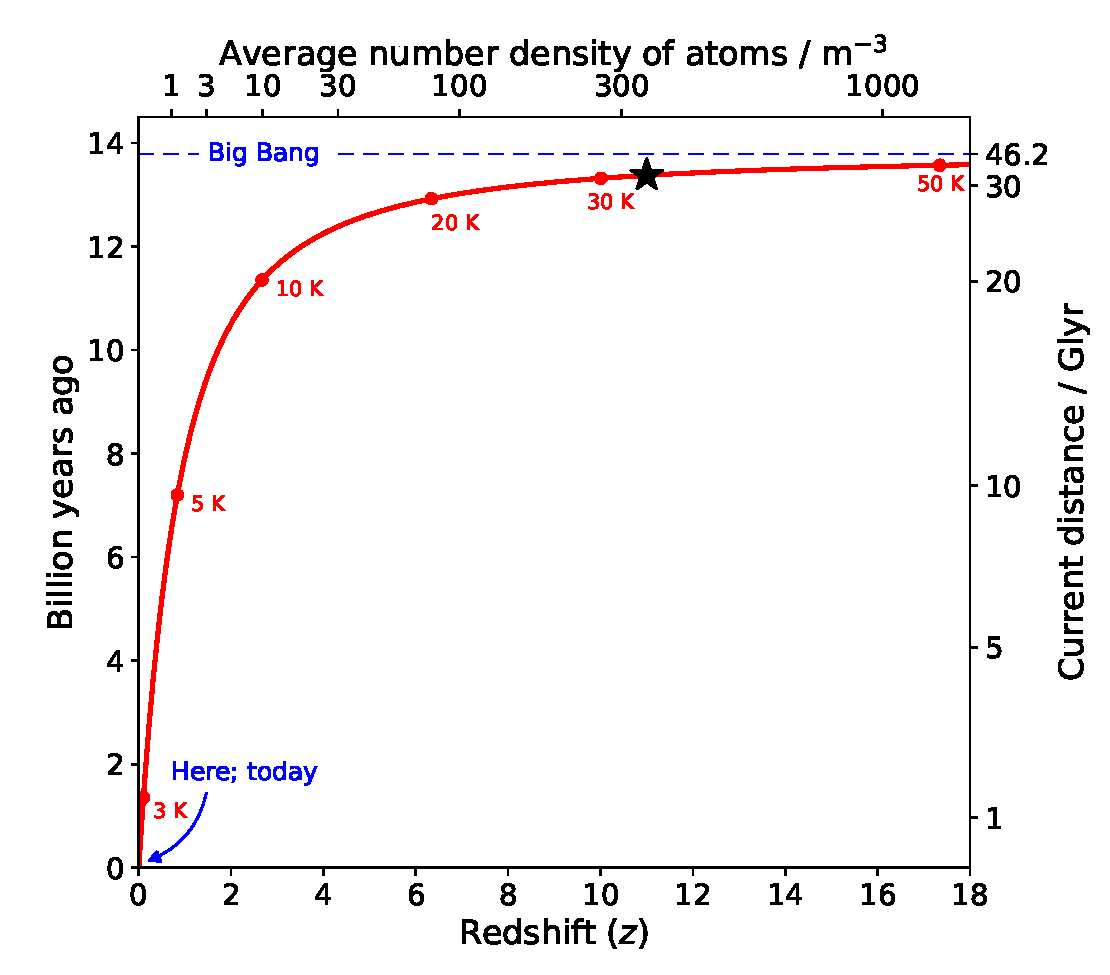
\includegraphics[width=0.98\linewidth]{redshift.pdf}
%         \caption{Relationship between the observed redshift of light emitted from a distant object (on the $x$ axis), and various properties of the Universe at the time the light was emitted:
%         Because the relative expansion was larger in the past when the Universe was smaller, redshift increased more then, asymptotically approaching infinity for light emitted at the time of the Big Bang, 13.8 Gyr ago.}
%         \label{fig:redshift}
%     \end{center}
% \end{figure}

% \begin{center}
% \pgfornament[width=.4\textwidth]{89}
% \end{center}

%%%%%%%%%%%%%%%%%%%%%%%%%%%%%%%%%%%%%%%%%%%%%%%%%%%%%%%%%%%%%%%%%%%%%%%%%%%%%%

% \section{Introduction}
% \label{sec:intro}

Lad os starte med konklusionen:
Det er en udbredt misforståelse --- selv blandt professionelle (og berømte) fysikere --- at vi ikke er i stand til at se galakser bevæge sig væk fra os med hastigheder større end lysets hastighed.
Eller sagt på matematisk, at vi ikke kan have --- eller i hvert fald ikke kan \emph{se} --- galakser med $\vrec > c$, hvor \vrec\ er galaksens hastighed i forhold til os, og $c$ er lysets hastighed.

Der er to måder at fortolke ``\emph{at se galakser bevæge sig med $\vrec>c$}'' på:
Fordi det tager tid for det lys, vi ser, at rejse ned til os, ser vi altid alle galakser, som de så ud i fortiden\footnote{Og det gælder sådan set ikke bare galakser, men også Solen, Månen og dit armbåndsur, som du ser henholdsvis 8 minutter, 1 sekund og 1 nanosekund tilbage i tiden.}.
Deres fart i dag er ikke den samme som den var i fortiden, så vi kan både spørge
\begin{formal}
    1. Kunne det lys, som vi ser fra en galakse, være blevet udsendt på et tidspunkt i fortiden, hvor hastigheden var $\vrec<c$, men i mellemtiden har Universets udvidelse accelereret, sådan at \emph{i dag} er $\vrec>c$?
\end{formal}
og
\begin{formal}
    2. Kunne galaksen virkelig have bevæget sig væk fra os med $\vrec>c$, da den udsendte det lys, vi set i dag?
\end{formal}

Især spørgsmål 2 menes ofte at være umuligt.
En variant af dette spørgsmål er
\begin{formal}
    2.1 Kan en galakse, som \emph{i dag} fjerner sig med $\vrec>c$, udsende en foton \emph{i dag}, som en eller anden dag i fremtiden når os?
\end{formal}

Svaret til alle tre spørgsmål er ``Ja''.

\section{Oprindelsen til misforståelsen}
\label{sec:oprindelsen}

Det er nok næsten almen viden, at intet kan bevæge sig hurtigere end lyset.
Denne forudsigelse af Einsteins relativitetsteori er blevet bekræftet eksperimentelt igen og igen.
Hvordan skulle det så være muligt for en galakse at bryde denne ``lov'', for slet ikke at tale om, hvordan vi skulle kunne se den?
\begin{figure}[!b]
    \centering
    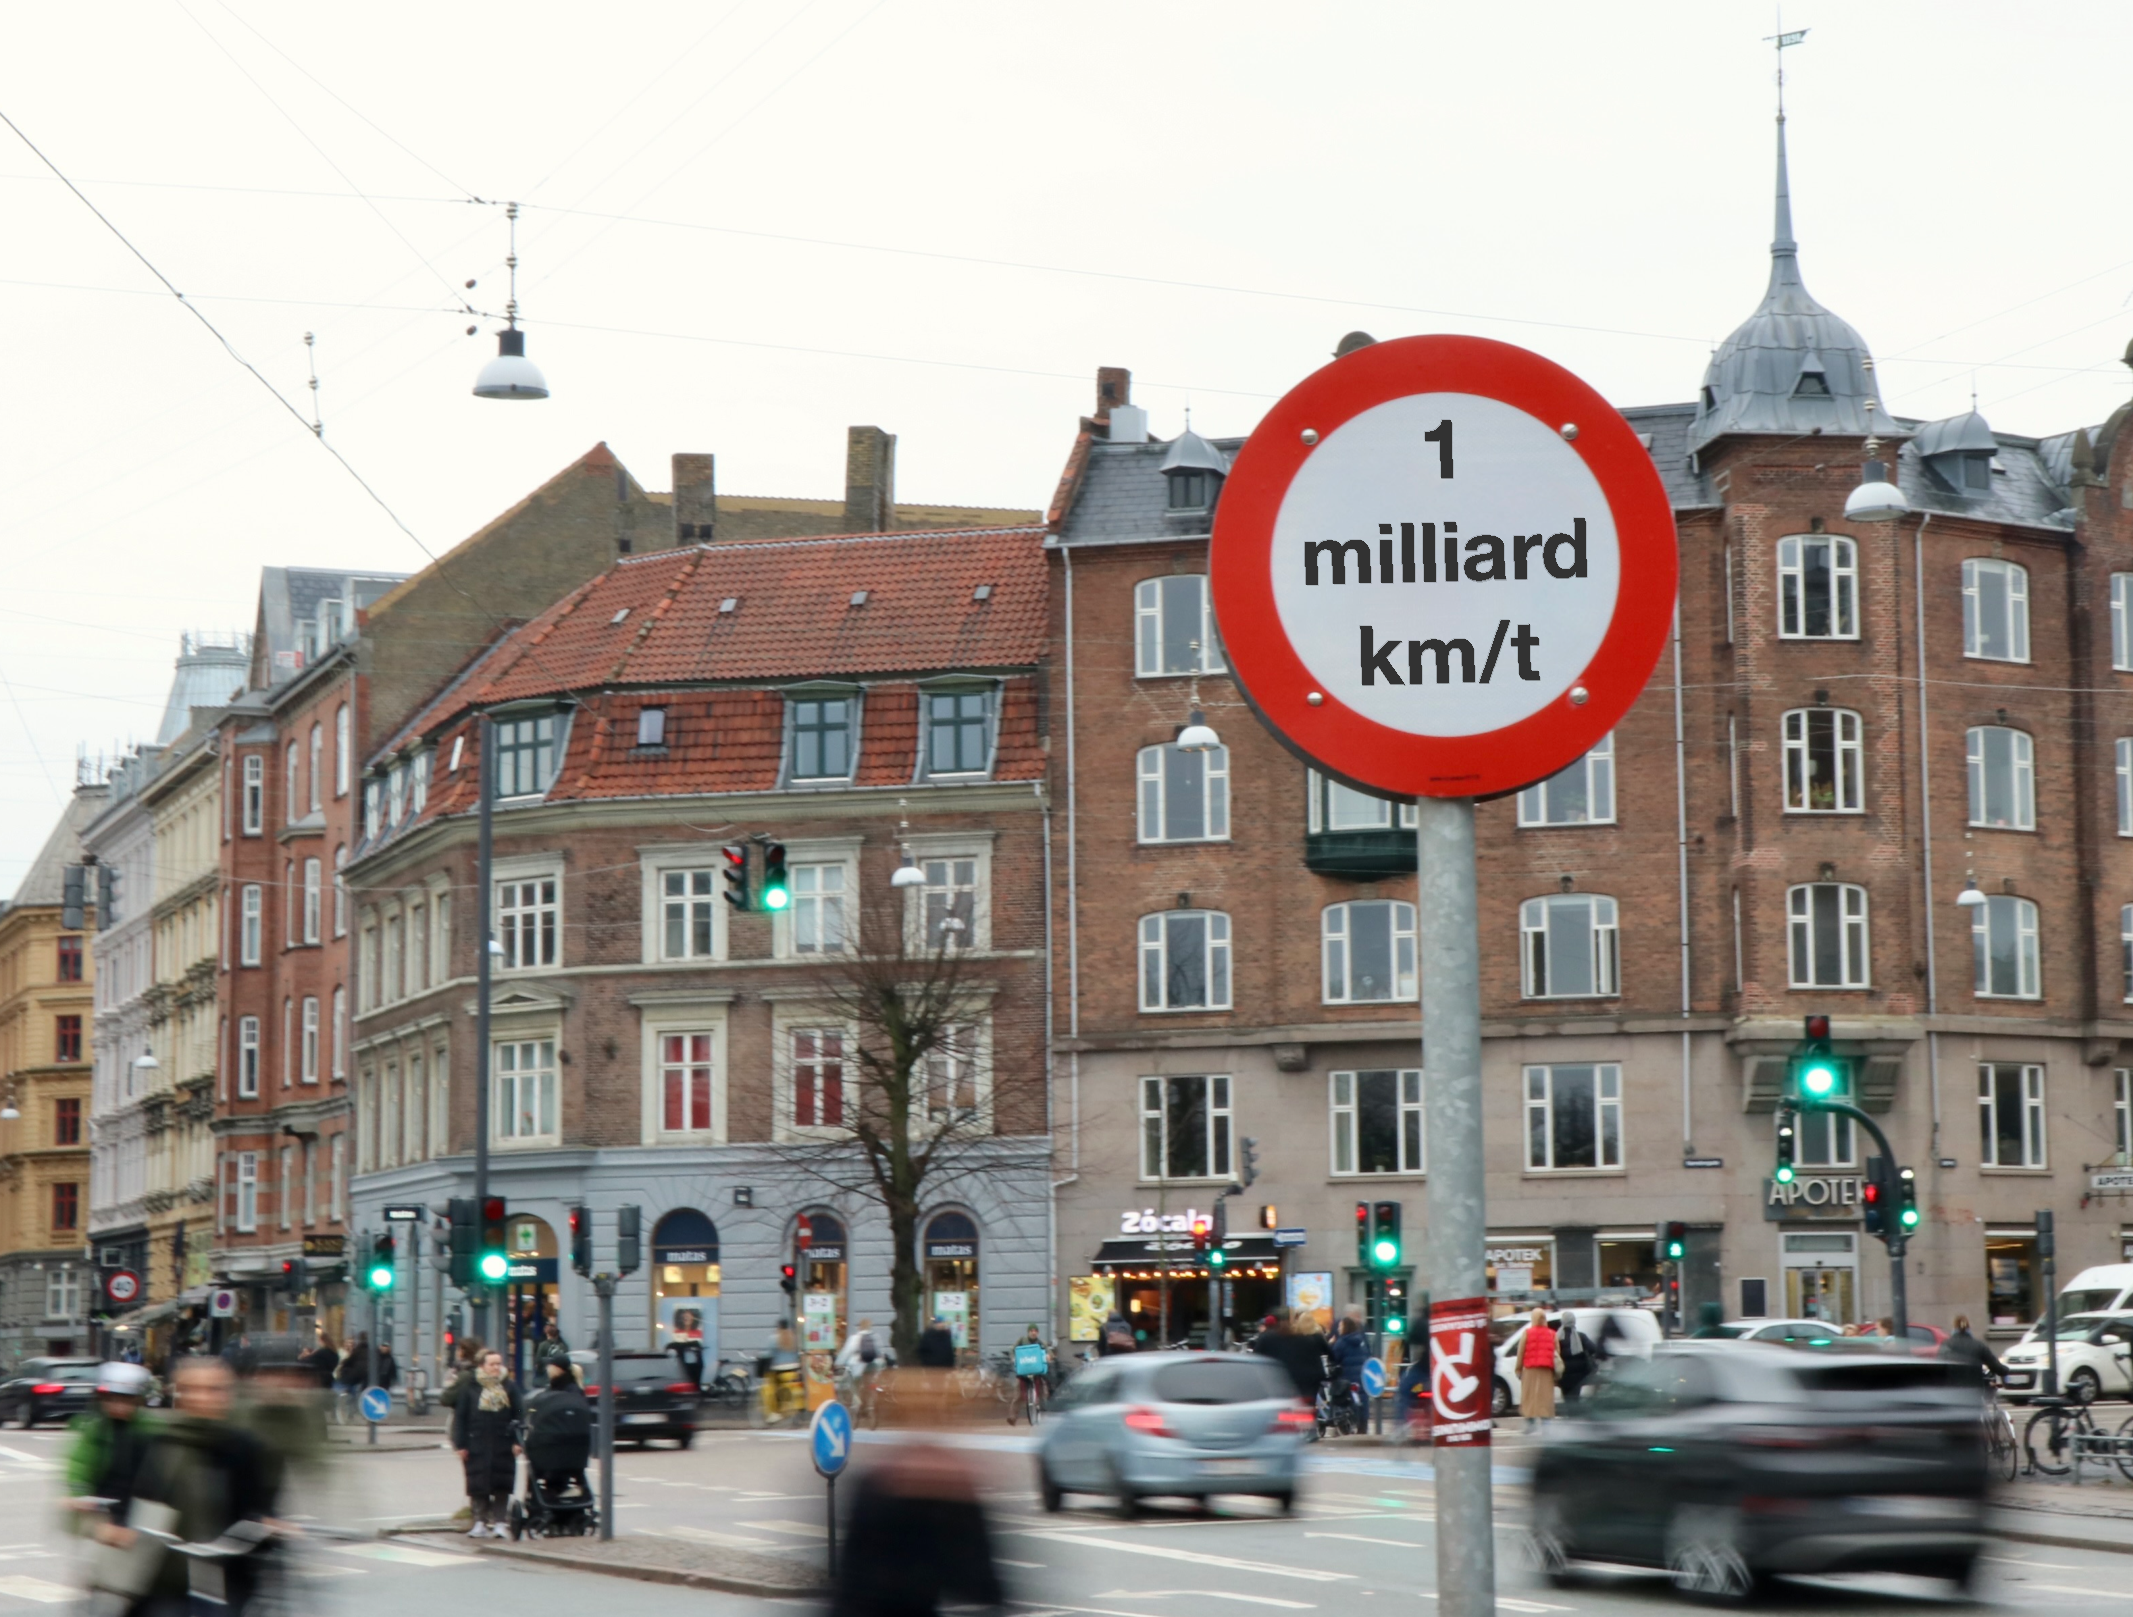
\includegraphics [width=0.45\textwidth] {./lysets-fart-skilt.pdf}
    \caption{\small{Lysets hastighed er præcis 299.792.458 m/s, men som astronom kigger dine kolleger mærkeligt på dig, hvis du ikke bare siger ``300.000 km/s''. Det svarer nogenlunde til en milliard km/t. Men er det virkelig en hastighedsbegrænsning? Foto(shop): Peter Laursen.}
    }
    \label{fig:c-skilt}
\end{figure}

Nøglen til at forstå dette tilsyneladende paradoks er, at den velkendte hastighedsgrænse er en forudsigelse af den såkaldte \emph{specielle} relativitetsteori \citep{Einstein1905}, som gælder \emph{bevægelse gennem rummet}:
To observatører i den samme, ikke-accelererede referenceramme (et såkaldt   \emph{inertialsystem}) kan ikke sende et signal til hinanden hurtigere end lyset.
Men galakserne bevægelse skyldes udvidelsen af selve Universet, som ikke er et inertialsystem, og som regeres af den \emph{generelle} (eller almene) relativitetsteori \citep{Einstein1916}.
Og her gælder andre regler.

\emph{Lokalt} kan intet rejse hurtigere end lyset, og lys rejser altid med $v=c$.
Så det gælder altså stadig, at intet kan overhale en lysstråle.
Men selve rummet kan udvide sig (eller trække sig sammen) så hurtigt eller langsomt, som det har lyst til, og kan dermed få to områder til at fjerne sig fra (eller nærme sig) hinanden med vilkårlig stor hastighed.

\section{Universets udvidelse}
\label{sec:udvidelse}

Mens galakser, som ligger i nærheden af hinanden, holdes sammen af deres gensidige tyngdekraft, ``trækkes'' fjernere galakser fra hinanden med en fart \vrec, som er proportional med deres afstand $d$.
Dette er essensen af Hubble--Lemaître-loven (som indtil 2018 var kendt som ``Hubble-loven'', men med 78\% stemmer mod 20\% blev anbefalet af den Internationale Astronomiske Union at få sit navn ændret, for at anerkende den belgiske præst og fysiker George Lemaîtres rolle i opdagelsen):
\begin{equation}
    \label{eq:hubble}
    \vrec = H_0 \, d.
\end{equation}
I denne ligning er $H_0$ en konstant, som kaldes Hubble-konstanten (men som vi vel nu burde kalde Hubble--Lemaître-konstanten?), der må bestemmes observationelt.
Hubble-konstanten udtrykkes i ``hastighed per afstand'', og fortæller altså, hvor hurtigt en galakse i en eller anden afstand $d$ fra os fjerner sig.
%
\begin{wrapfigure}{l}[20pt]{.25\textwidth}
    \caption*{{\sf \color{darkgreen}{
        Afstande i Universet kan måles i lysår, men i astronomi bruges normalt \emph{parsec}, som er ca. 3,26 lysår.
        Store afstande måles gerne i millioner af parsec, dvs. megaparsec, forkortet Mpc.
    I denne artikel holder vi os dog mest til lysår.
    \vspace{-5mm}
}}}
\end{wrapfigure}
%
Hubble-konstanten har en værdi på omkring\footnote{En lille, men betydelig og uafklaret, forskel fås, alt efter hvilken metode man bruger til at måle $H_0$. Om denne såkaldte ``Hubble tension'' kan du læse i en artikel, jeg skrev for nylig på \href{https://videnskab.dk/rummet/hvilken-hastighed-udvider-universet-sig-med}{videnskab.dk/rummet/hvilken-hastighed-udvider-universet-sig-med}.} 
$H_0 \simeq 70 \,\mathrm{km}/\mathrm{s}/\mathrm{Mpc}$.
Det vil sige, at en galakse, der ligger f.eks. 100 Mpc væk, fjerner sig fra os med 7.000 km/s, mens en galakse, der ligger 200 Mpc væk, fjerner sig med 14.000 km/s.

Sådan en udvidelse kaldes \emph{homolog}, og er blevet sammenlignet med en rosinbolle:
Efterhånden som gæren får bollen til at hæve, øges afstanden mellem to rosiner med en fart, som er proportional med deres indbyrdes afstand på et givet tidspunkt.
Jo større afstanden bliver mellem to rosiner, jo hurtigere fjerner de sig fra hinanden.
Det samme sker med galakser i rummet, og for store nok afstande overstiger den hastighed, de fjerner sig med, lysets fart.

Dette overtræder ikke relativitetsteorien, som kun siger, at intet kan rejse \emph{gennem} rummet med $v>c$.
Galakserne rejser godt nok også gennem rummet, sådan lidt hid og did, fordi de påvirker hinanden med deres tyngdekraft.
Alt efter hvor store grupper de ligger i, giver dette anledning til såkaldte ``egenbevægelser'' med nogle 100 eller 1000 km/s.
Men det kosmologiske Hubble-flow er anderledes; man kan sige, at rummet udvider sig og ``trækker'' galakserne med sig (selv om nogle ikke bryder sig om denne formulering), sådan at deres afstand til os, og til hinanden, øges.
Hvorvidt denne bevægelse i virkeligheden kan kaldes ``en hastighed'' er blevet debatteret \citep[f.eks.][]{Harrison2000}, men begrebet overholder trods alt den normale definition for hastighed, dvs. ``hvor hurtigt ændrer positionen (eller afstanden) sig?''.

En måske mere beskrivende analogi fås, hvis vi stepper en dimension ned, og betragter den todimensionale overflade på en ballon, hvorpå der kravler nogle myrer rundt (se Fig.~\ref{fig:ballon}).
\begin{figure}[!t]
    \centering
    \includegraphics [width=0.45\textwidth] {./ballon.pdf}
    \caption{\small{
        Til venstre ses en let slatten ballon med tre myrer på, som hedder Alice (\emph{rød}), Bob (\emph{sort}) og Carlos (\emph{orange}).
        Alice og Bob er 10 cm fra hinanden, mens Carlos ligger 5 cm og 7 cm fra hhv. Alice og Bob.
        Til højre har jeg pustet ballonen op til dobbelt størrelse.
        Bob er nu 20 cm fra Alice, og hvis jeg havde pustet hurtigt nok, vil jeg kunne få Bob og Alice til at fjerne sig fra hinanden med over-myrehastighed.\\
        Alle afstande fordobles, når ballonens diameter fordobles, så Carlos ligger nu 10 cm og 14 cm fra hhv. Alice og Bob.
        Myrerne selv tager dog ikke del i denne udvidelse, da elektromagnetiske kræfter holder sammen på deres exoskelet, og på samme måde vokser galakser heller ikke med Universet, da tyngdekraften holder sammen på dem.
        Alle tre myrer tænker, at de ligger stille, mens de to andre fjerner sig, og derfor tror de, at de sidder i midten af ballonens overflade.
        Skøre myrer.\\
        Foto: Peter Laursen.}
    }
    \label{fig:ballon}
\end{figure}
Myrerne i vores eksempel er lidt sløve i det, og kravler rundt med max 1 cm/s, så to myrer kan altså ikke umiddelbart komme hurtigere væk fra hinanden end med 2 cm/s.
%
\begin{wrapfigure}{r}[20pt]{.25\textwidth}
    \caption*{{\sf \color{darkgreen}{
Ballonen er også god til at vise, hvordan alle afstande vokser med den samme faktor.
Men man skal ikke tage den alt for seriøst, for hvor ballonens 2D-overflade udvider sig i et 3D-rum, udvider vores 3D-Univers sig ikke i nogen højere dimension.
Man kan sige, at det ``udvider sig i sig selv''; selve geometrien udvikler sig sådan, at afstande ændres.
    \vspace{-5mm}
}}}
\end{wrapfigure}
%
Men hvis du giver dig til at puste ballonen op alt hvad du kan, kan du få afstanden mellem to myrer til at øges med f.eks. 10 cm/s.
Og jo længere der er mellem to myrer, jo hurtigere fjerner de sig fra hinanden.
%Uanset hvordan man formulerer det, er det dog et faktum, at afstanden til nogle galakser vokser hurtigere end lysets fart.
På samme måde kan galakser godt fjerne sig fra hinanden hurtigere end lysets fart, selvom hverken de eller fotoner kan bevæge sig gennem rummet hurtigere end lysets.

% \noindent\fcolorbox{darkgray}{lightgray}{%
\begin{figure}[!t]
\minipage[t!]{\dimexpr0.98\linewidth-2\fboxsep-2\fboxrule\relax}
\begin{bclogo}[
    couleur=gray!20,
    epBord=1,
    arrondi=0.1,
    logo=\bcinfo,
    marge=8,
    ombre=false, %true,blur,
    couleurBord=gray!60,
    barre=line]
    { \ \textsf{Observationelle faldgruber}}
    \small{\textsf{
        Selvom ligning~\ref{eq:hubble} antyder en lineær sammenhæng mellem afstand og hastighed, er hverken \vrec\ eller $d$ noget, som er sådan lige til at måle.
        Man kan (i nogle tilfælde) måle \emph{rødforskydningen} $z$ af en galakse, dvs. hvor meget den spektrum er blevet forskudt.
        For nære galakser fortæller det os, at hastigheden er $\vrec\simeq cz$, men allerede for $z\gtrsim0,\!01$ bliver denne relation unøjagtig.
        For større rødforskydninger kan den speciel-relativistiske formel bruges, men fordi Universets udvidelseshastighed har ændret sig gennem tiden, bliver dén også unøjagtig ved $z\gtrsim0,\!1$.
        For endnu større rødforskydninger er man nødt til at kosntruere en model for Universets dynamik.
        Standardmodellen er den såkaldte Friedmann--Lemaître---Robertson--Walker-metrik \citep{Friedmann1922,Lemaitre1927,Robertson1935,Robertson1936a,Robertson1936b,Walker1937}, som sammen med ``det kosmologiske princip'' --- dvs. den antagelse, at Universet på store nok skalaer er \emph{homogent} (dvs. ens over det hele) og \emph{isotropt} (dvs. ens i alle retninger) --- giver den såkaldte \emph{Friedmann-ligning}, der beskriver hvordan udvidelseshistorien er dikteret af, hvor meget der er af Universets forskellige komponenter: mørkt stof, normalt stof, mørk energi og stråling.\vspace{1mm}\\
        En anden bekymring er, hvordan man beregner afstande.
        Eftersom vi ikke kan måle dem direkte, gør vi brug af såkaldte \emph{standard-lyskilder}, dvs. objekter som vi ved, hvor meget lys udsender, og sammenligner med, hvor meget lys vores teleskoper opfanger.
        Da deres lys har rejst gennem det ekspanderende Univers, benytter vi igen Friedmann-ligningen for at få sammenhængen mellem det udsendte lys, det observerede lys, og afstanden.
    }}
\label{info:obs-faldgrube}
\end{bclogo}
     \endminipage
     %}\hfill
\end{figure}

\section{Hubble-sfæren og partikelhorisonten}
\label{sec:dH-dP}

Som nævnt ovenfor medfører ligning~\ref{eq:hubble}, at for tilstrækkeligt store $d$, vil \vrec\ overstige lysets hastighed, og det er ligetil at beregne denne såkaldte Hubble-længde til
\begin{equation}
    \label{eq:dH}
    d_\mathrm{H} = \frac{c}{H_0}
                \simeq 4400\,\mathrm{Mpc}
                \simeq 14,4\,\mathrm{mia.\,lysår}.
\end{equation}
Indenfor denne ``grænse'' fjerner galakser sig langsommere end $c$ (også kaldet ``subluminalt''), og udenfor fjerner de sig hurtigere (``superluminalt'').
Området indenfor kaldes for ``Hubble-sfæren'' (eller måske ``Hubble--Lemaître-sfæren''? Okay, jeg stopper nu), men der er altså ikke noget særligt ved hverken galakserne indenfor eller udenfor.

Som tiden går, ser vi fjernere og fjernere galakser, efterhånden som deres lys når ned til os.
Det fjerneste vi i princippet kan se --- altså dét, der ligger så langt væk, at lyset derfra har brugt hele Universets levetid på at nå os --- kaldes \emph{partikelhorisonten}, og afstanden $d_\mathrm{P}$ til denne horisont vokser altid, både fordi tiden går (så fjernere lyskilder bliver synlige), og fordi rummet udvider sig.
Hvis rummet \emph{ikke} udvidede sig, ville partikelhorisonten være 13,8 mia.~lysår væk (fordi Universet er 13,8 mia.~år gammelt), men udvidelsen har båret horisonten væk til en nuværende afstand på $d_\mathrm{P} =$ 46,3 mia.~lysår.
Den del af Universet, som ligger indenfor partikelhorisonten, kalder vi ``det observerbare Univers'', og udenfor den kugleformede del af Universet, som vi altså kan se, ligger der formodentlig meget mere Univers, måske endda uendelig meget.
%
\begin{wrapfigure}{l}[20pt]{.25\textwidth}
    \caption*{{\sf \color{darkgreen}{
        Vi opdager rutinemæssigt galakser både 20 og 30 mia.~lysår væk.
        I skrivende stund indehaves afstandsrekorden af JADES-GS-z13-0, en galakse der ligger 33 mia.~lysår væk \citep{Curtis-Lake2023}.
        På grund af lysets lange rejsetid ser vi den, som den så ud for 13,5 mia.~år siden, da Universet var blot 300 millioner år gammelt.
        \vspace{-5mm}
}}}
\end{wrapfigure}
%
Vi ser dem altid, som de så ud i fortiden, for milliarder af år siden.
Men hvad hvis vi vil vide, hvordan de ser ud \emph{i dag}?
Ville nogle af disse galakser kunne udsende noget lys, som vi kan opfange en dag ude i fremtiden?

Måske har du hørt, at Universet ikke bare udvider sig, men også \emph{accelererer} i sin udvidelse.
Men lad os først betragte et (hypotetisk) univers (med lille u, fordi det ikke er \emph{vores} Univers), som bare udvider sig uden acceleration.
Det er en kontraintuitiv kendsgerning --- men ikke desto mindre en kendsgerning --- at der i et sådan univers ingen grænse er for den afstand vi kan se, hvis vi bare venter længe nok.
Uanset hvor fjern en galakse er, og dermed hvor hurtigt den fjerner sig fra os, selv nok så superluminalt, kan den udsende en foton, som en dag i en fjern fremtid vil nå os, omend det kan tage milliarder af milliarder af år.

\section{En myre på en elastik}
\label{sec:myre}

Dette tilsyneladende paradoks kan beskrives i en analogi, hvor problemet omformuleres til en myre, som kravler afsted med 1 cm/s, langs et elastikbånd som strækkes med 1 \emph{meter} i sekundet (så altså, for at være eksplicit, så er elastikken en analogi for Universet, og myren er en analogi for en foton).
Den ene ende af elastikken fastgøres til en mur, og her starter myren; den anden ende tager du fat i, og løber væk.
Vil myren nogensinde kunne nå dig for enden af elastikken?
Utroligt nok viser det sig, at ja, det kan den.

At løse dette problem kræver lidt matematik, som du kan hygge dig med i infoboks~\ref{info:myre} hvis du har lyst, men en intuitiv måde at få hovedet rundt om det på er at betragte myren fra startpunktet (muren) i stedet for målet (dig).
Myren starter ud med en hastighed på 1 cm/s, men som den øger sin afstand til muren, får den ekspanderende elastik myrens hastighed ift. muren til at stige.
Eftersom udvidelsen er den samme langs hele elastikken, udvider den sig både foran og bagved myren.
Det vil altså sige, at på et hvilket som helst tidspunkt under rejsen, er \emph{andelen} af den totale distance, som myren har tilbagelagt, uafhængig af udvidelseshastigheden, og uanset hvor stor denne udvidelseshastighed er, stiger andelen kontinuerligt fra 0 til 1.
Denne sidste sætning indeholder løsningen på ``paradokset'', så læs den lige igen.

Som tiden går, stiger andelen langsommere og langsommere, og det er måske ikke så intuitivt, at summen --- eller rettere \emph{integralet} --- af de individuelle skridt, nogensinde vil nå 1.
For at se dette, er vi nødt til at udføre den formelle matematiske løsning.

% \noindent\fcolorbox{darkgray}{lightgray}{%
\begin{figure*}[!t]
    \centering
\minipage[t!]{\dimexpr0.98\linewidth-2\fboxsep-2\fboxrule\relax}
\begin{bclogo}[
    couleur=gray!20,
    epBord=1,
    arrondi=0.1,
    logo=\bcinfo,
    marge=8,
    ombre=false, %true,blur,
    couleurBord=gray!60,
    barre=line]
    { \ \textsf{Myren på elastikbåndet: matematisk bevis}}
    \small{\textsf{
        I følgende bevis vil vi måle myrens position på to forskellige måder; både med koordinater $x$ ift. jorden, og som andelen $\chi$ (det græske bogstav \emph{chi}) af elastikken.
        Vi kan jo kalde dem hhv. jord-koordinater og elastik-koordinater.\vspace{1mm}\\
        Bind den ene ende af elastikbåndet fast til en mur, hold fast i den anden ende, og start så, når klokken er $t=0$, ved positionen $x=x_0$ med at hive i enden med hastigheden $v$.
        Lad samtidig (dvs. til $t=0$) myren starte med at kravle med hastigheden $\omega$ (det græske bogstav \emph{omega}) i forhold til båndet, fra $\chi=0$ (som falder sammen med $x=0$) henimod $\chi=1$ (som er elastik-koordinaten for den ende du holder i).
        Den afgørende del er at indse, at uanset hvor hurtigt elastikkens ende trækker sig væk fra myren, så stiger myrens position i termer af $\chi$ altid ($x$ stiger også, men \emph{din} $x$-værdi stiger hurtigere, så det fortæller os ikke så meget).
    \begin{center}
        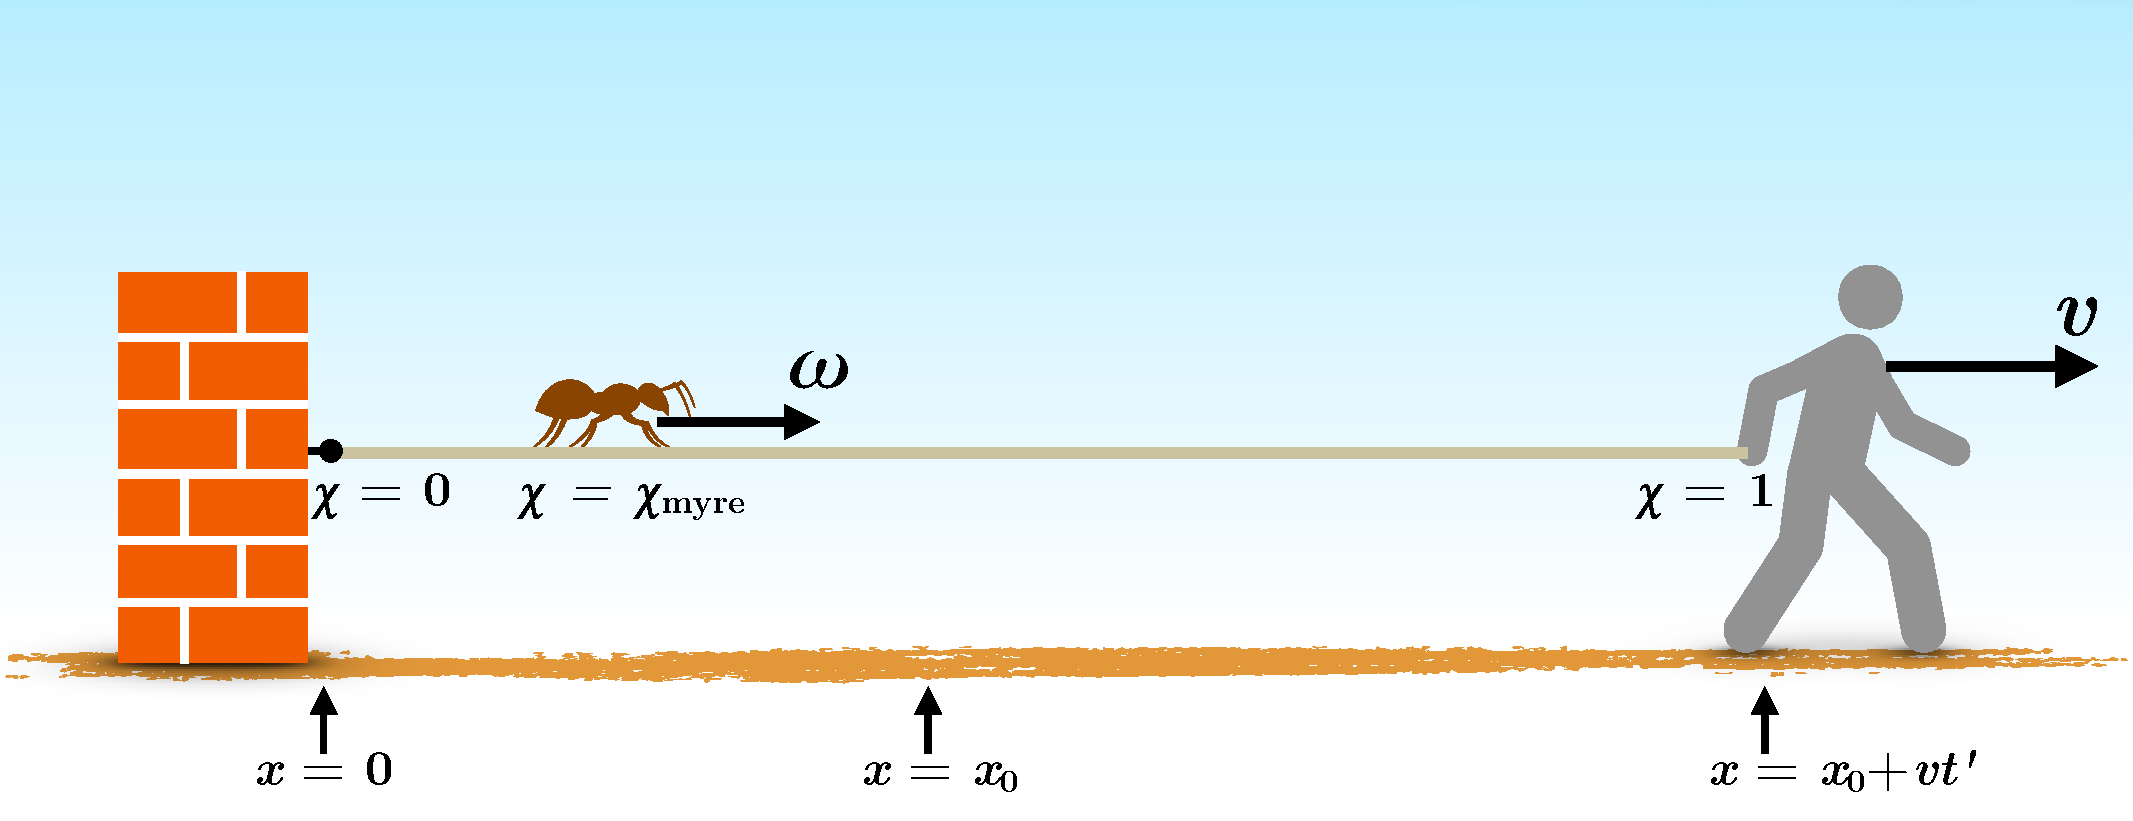
\includegraphics [width=0.75\textwidth] {./ant-on-a-rubber-rope.pdf}
    \end{center}
    På et senere tidspunkt $t$ er båndet blevet strukket til en længde $x = x_0 + v t$.
    Myren fortsætter med at øge sin tilbagelagte andel $\chi_\mathrm{myre}$, men hastigheden som denne andel stiger med, falder omvendt proportionalt med længden af båndet:
    \begin{equation}
        \label{eq:dchi_dt}
        \frac{d\chi_\mathrm{myre}}{dt} = \frac{\omega}{x_0 + v t}.
    \end{equation}
    Ved integration af ligning~\ref{eq:dchi_dt} kan vi finde den tilbagelagte andel til tiden $t$:
    \begin{eqnarray}
        \label{eq:chit}
        \nonumber
        \chi_\mathrm{myre}(t) & = & \int_0^{t} \frac{\omega}{x_0 + v t'} \, dt'\\
                              & = & \frac{\omega}{v} \ln \left(1+\frac{vt}{x_0}\right).
    \end{eqnarray}
    Hvis der er en tid $t_\mathrm{slut}$, hvor myren når elastikkens ende, så må det gælde, at $\chi_\mathrm{myre}(t_\mathrm{slut}) = 1$.
    Fra ligning~\ref{eq:dchi_dt} må vi derfor have, at
    \begin{equation}
        \nonumber
        1 = \frac{\omega}{v} \ln\left(1+\frac{vt_\mathrm{end}}{x_0}\right),
    \end{equation}
    eller
    \begin{equation}
        \label{eq:tend}
        t_\mathrm{end}=\frac {x_0}{v}\left(e^{v/\omega}-1\right).
    \end{equation}
    Hvis for eksempel myren kravler med $\omega = 1$ cm/s, du starter ved $x_0 = 1$ meter, og trasker afsted med $v = 1$ m/s, så fås fra ligning~\ref{eq:tend}, at myren når dig efter en tid $t_\mathrm{slut} = (e^{100}-1)$ sekunder, eller knap en billion billiarder år --- langt, langt længere tid end Universets nuværende alder.
    \vspace{1mm}\\
    Løsningens eksponentielle natur gør, at forholdet mellem myrens og din hastighed har stor betydning for resultatet:
    Hvis myren kravler 10 gange hurtigere --- dvs. med $\omega = 10$ cm/s --- når den dig efter kun godt 6 timer, mens hvis den kravler med 4 mm/s, tager det en googol år.
    \vspace{1mm}\\
    Men pointen med denne øvelse var ikke så meget det præcise resultat som det faktum, at uanset hvad forholdet er mellem hastighederne, så er det i princippet altid muligt for myren at indhente dig, så længe du ikke accelererer.
    }}
\label{info:myre}
\end{bclogo}
     \endminipage
     %}\hfill
\end{figure*}

\section{Den kosmiske begivenhedshorisont}
\label{sec:dE}
I tilfælde af, at du sprang infoboks~\ref{info:myre} over (hvilket jeg ikke vil holde dig op på), vil jeg bare lige gentage pointen:
Uanset hvor langsomt en myre kravler på et elastikbånd, og uanset hvor hurtigt du strækker det, vil myren en dag nå dig, hvis du altså strækker det med \emph{jævn} fart (vi ser her bort fra kedelige biologiske processer som f.eks. din og myrens levetid, og andre forstyrrende fakta).
Det samme princip gælder i det ekspanderende Univers:
Hvis Universet udvidede sig med jævn fart, så ville der ikke være nogen grænse for, hvor fjerne galakser vi kunne se, hvis bare vi ventede længe nok.

Desværre er vores Univers ikke helt så simpelt; observationer af udvidelseshastigheden gennem Universets historie viser os, at det i starten udvidede sig meget hurtigt, mens det langsomt bremsedes op pga. den gensidige tyngdekraft af alt det stof (og stråling) der nu engang ligger rundt omkring.
Men efter omkring 10 mia.~år begyndte det på mærkværdigvis at accelerere i sin udvidelse.
Vi forstår ikke rigtig hvorfor, og vores bedste bud indtil videre er en form for mystisk egenskab ved selve det tomme rum, som vi for at lyde lidt dramatiske kalder for \emph{mørk energi}.

Uanset hvad det skyldes, betyder denne acceleration at der \emph{er} grænse for, hvor langt vi kan se.
For en galakse længere væk end en bestemt afstand $d_\mathrm{B}$, kendt som \emph{den kosmiske begivenhedshorisont}, er den den triste sandhed, at hvis den udsender en lysstråle i dag, så vil vi aldrig se den.
På grund af accelerationen bevæger galakserne sig efterhånden ud på den anden side af denne horisont.
Med andre ord, som tiden går, vil flere og flere galakser \emph{ikke} være i stand til at sende nye signaler til os.
Vi kan stadig se dem, men vi ser dem som de så ud i fortiden, dvs. vi ser fotoner som blev udsendt for længe siden.

Afstanden til den kosmiske begivenhedshorisont kan beregnes ved et integrale, der involverer den såkaldte Friedmann-ligning, som afhænger af tætheden af Universets komponenter\footnote{Hvis du virkelig insisterer på at få ligningen, er den givet ved
% $$
% d_\mathrm{B}(t) = a(t) \int_t^\infty \frac{c\,dt'}{a(t')},
% $$
$d_\mathrm{B}(t) = c a(t) \int_t^\infty a^{-1}(t')dt$,
hvor ``skala-faktoren'' $a(t)$, som beskriver udvidelsen og er defineret til $a(\mathrm{i\,dag}) = 1$, er givet ved
$H^2(a)/H_0^2 = \Omega_\mathrm{r}a^{-4} + \Omega_\mathrm{M}a^{-3} \Omega_k a^{-2} + \Omega_\Lambda$,
% $$
% \frac{H^2(a)}{H_0^2} =
% \frac{\Omega_\mathrm{r}}{a^4} +
% \frac{\Omega_\mathrm{M}}{a^3} +
% \frac{\Omega_k}{a^2} +
%       \Omega_\Lambda,
% $$
hvor $\{\Omega_\mathrm{r}, \Omega_\mathrm{M}, \Omega_\Lambda\} \simeq \{\lesssim10^{-4},0.3,0,0.7\}$ er andelen af energitæthederne af hhv. stråling, stof og mørk energi, mens $\Omega_k\simeq$ beskriver Universets overordnede krumning. Held og lykke med at regne dén ud uden en computer.}, og er i dag
\begin{equation}
    \label{eq:dB}
        d_\mathrm{B} = 16,\!3\,\mathrm{mia.\,lysår}.
\end{equation}

% \section{Den ``superlumino-observerbare kugleskal''}
% \label{sec:obsskal}

% Ligning~\ref{eq:dH} fortalte os, at alle galakser, der ligger længere væk end $d_\mathrm{H} =$ 14,4 mia.~lysår, fjerner sig hurtigere end lysets fart.
% Samtidig fortæller ligning~\ref{eq:dB} os, at galakser, der ligger nærmere end $d_\mathrm{B} = $ 16,3 mia.~lysår vil kunne udsende en foton i dag, som vi vil kunne se i en fjern fremtid.
% % Og dét på trods af, at de og Mælkevejen fjerner sig fra hinanden med en fart, som overstiger lysets.
% Alle galakser, der ligger mellem disse horisonter gør os i stand til at kunne sige ``Ja, der findes galakser, som bevæger sig hurtigere væk fra os end lysets hastighed, men som vi alligevel kan se, ikke bare som de så ud i fortiden, men som de ser ud i dag, hvis vi bare har tålmodighed''.

Figur~\ref{fig:horizons} illustrerer de forskellige horisoner ift. os.
\begin{figure*}[!t]
    \centering
    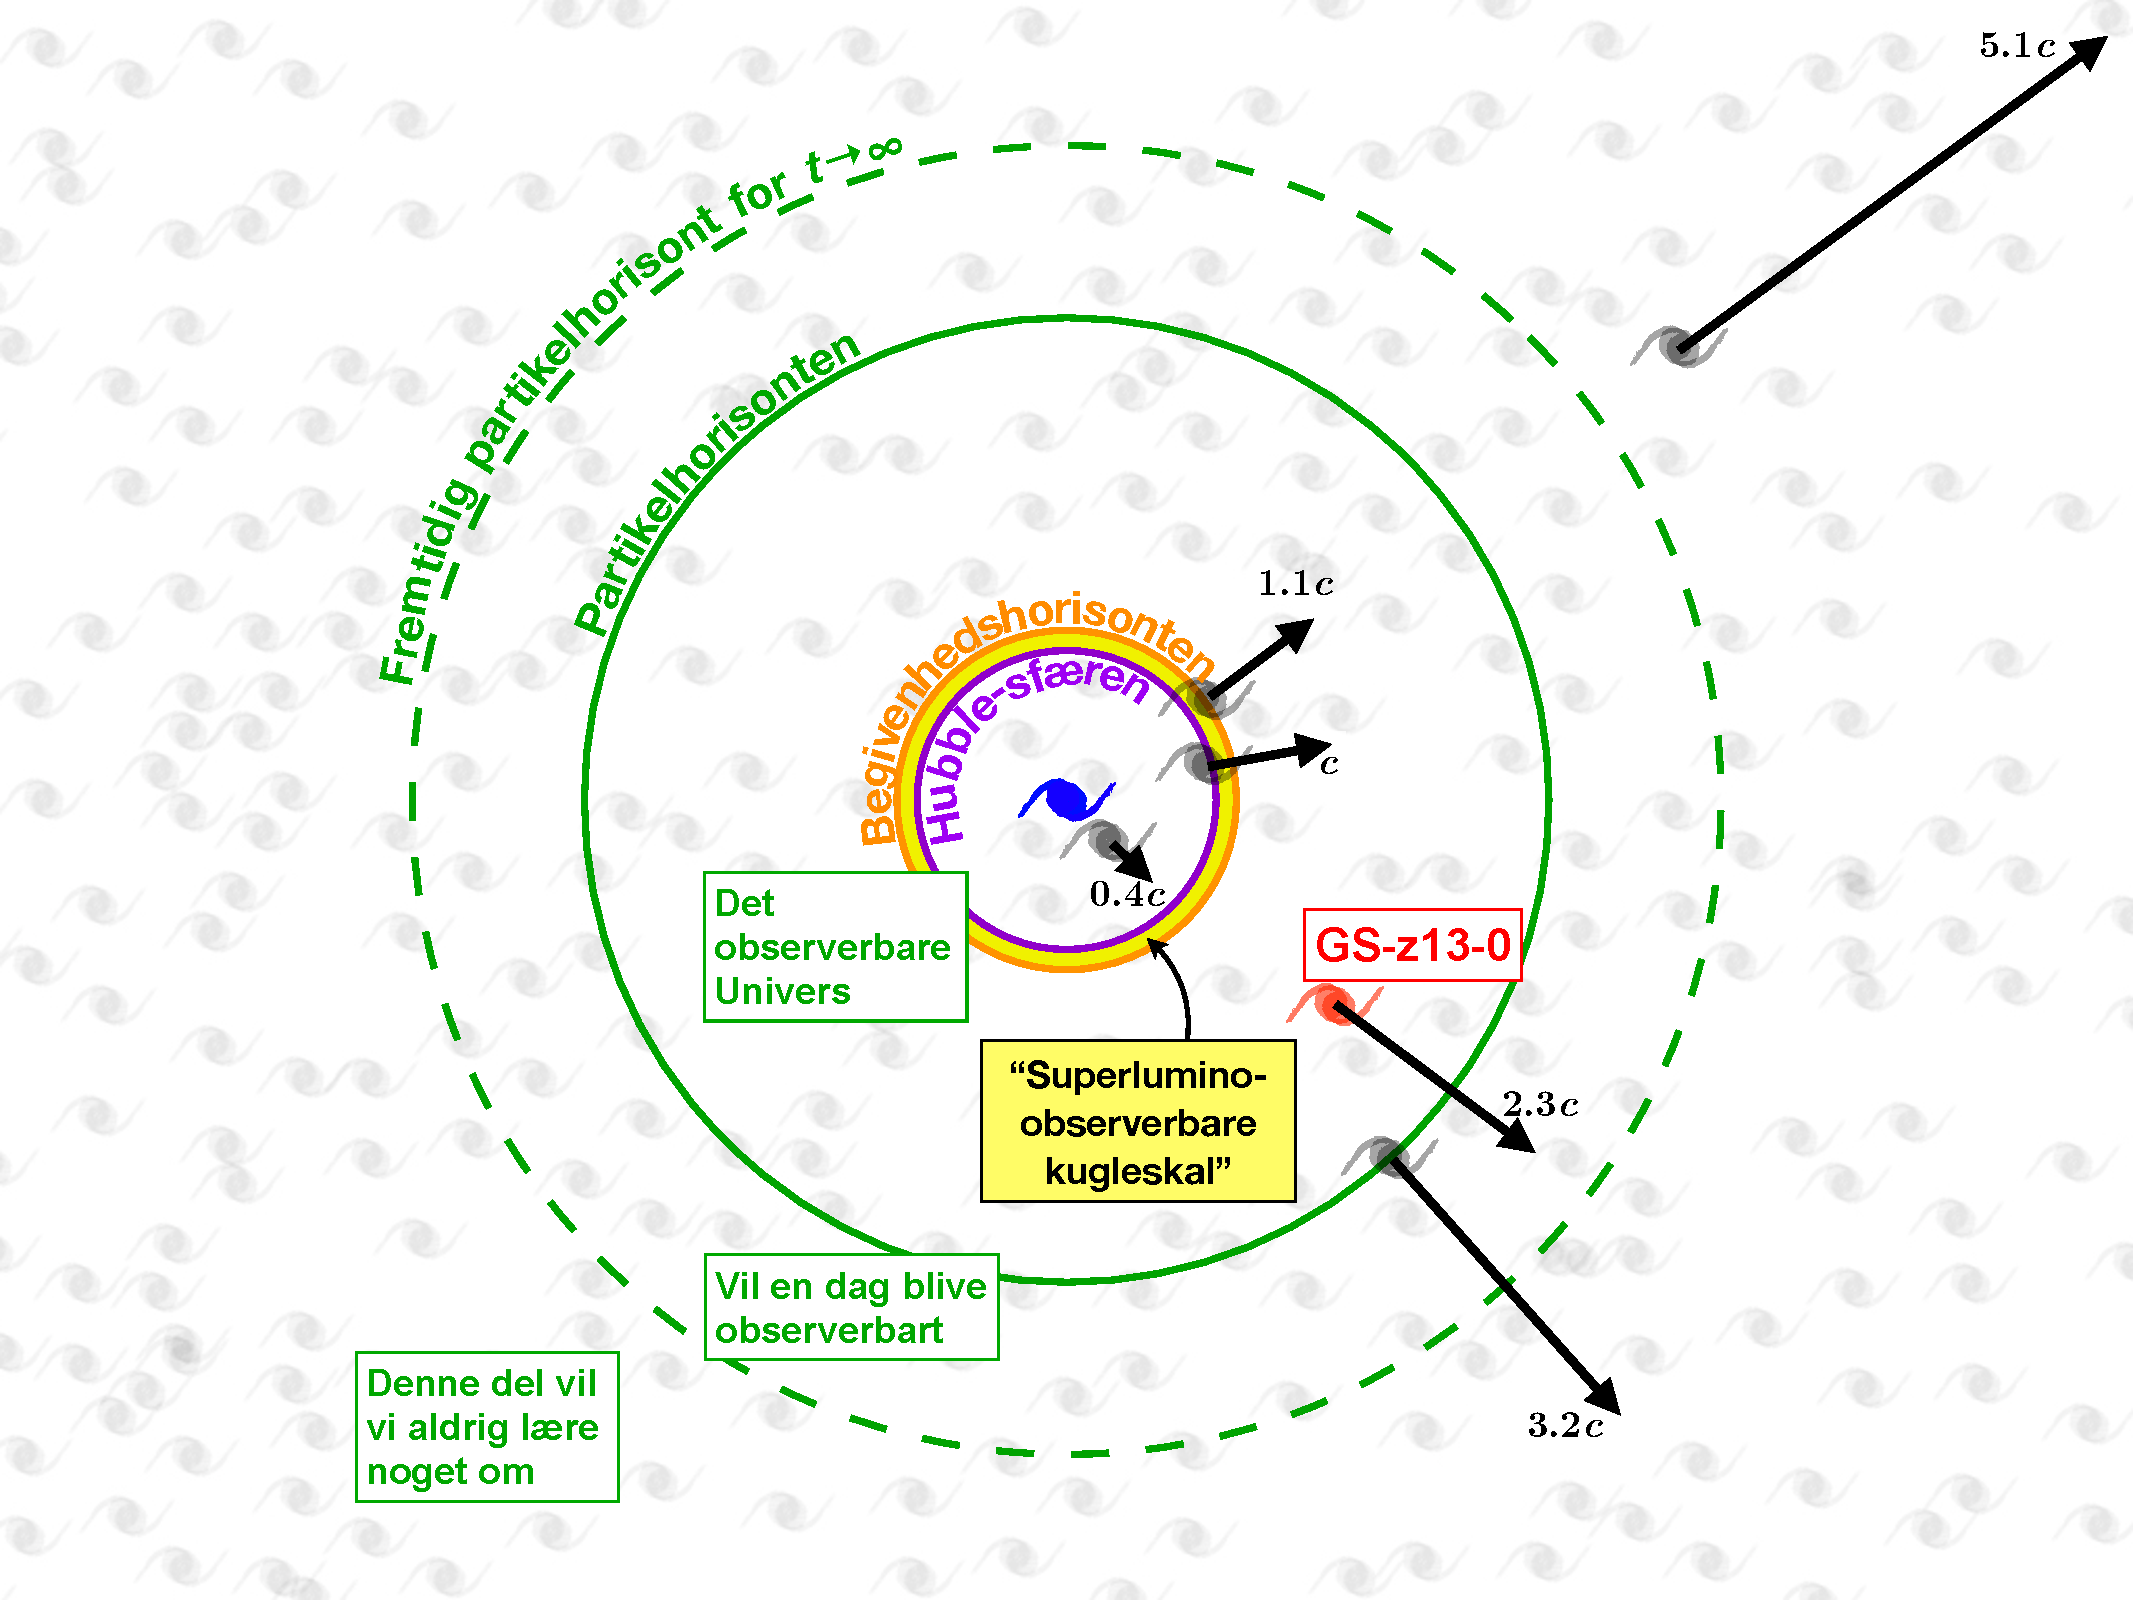
\includegraphics [width=0.90\textwidth] {./horizons.pdf}
    \caption{\small{
        Et snapshot af Universet i dag, centreret på Mælkevejen (blå).
        Galakser (grå) ligger spredt ud over det hele, måske i al uendelighed.
        De fjerner sig alle fra hinanden proportionalt med deres indbyrdes afstand; nogle få (mørkegrå) har deres fart indikeret.
        Den fjerneste galakse vi kendes, JADES-GS-z13-0, fjerner sig med 2.3 gange lysets fart.
        Så længe de er indenfor partikelhorisonten (grøn solid) kan vi dog alligevel se dem, selvom vi altid ser dem i fortiden.
        Hvis vi vil se, hvordan de ser ud i dag, må vi vente, men så længe de ligger indenfor begivenhedshorisonten, er det ikke noget problem, så længe vi er tålmodige; deres lys skal nok kunne nå os.
        Den tynde, gule skal mellem Hubble-sfærens kant (lilla) og begivenhedshorisonten indeholder dermed galakser (omkring 10 milliarder), som fjerner sig hurtigere end lysets fart, men som vi alligevel kan se.
        Ligger de længere væk, vil Universets acceleration dog bære lyset væk fra os for hurtigt til, at det kan overkomme udvidelsen.
        I fremtiden vil lyset fra fjernere galakser nå os, sa partikelhorisonten vokser, men igen sætter accelerationen en stopper for spasen, idet den aldrig vil vokse længere ud end de galakser, som i dag er 62.8 mia.~lysår væk (men som altså i fremtiden kommer længere og længere væk med eksponentielt stigende hast. Illustration: Peter Laursen.)
    }}
    \label{fig:horizons}
\end{figure*}
\section{Den ``superlumino-observerbare kugleskal''}
\label{sec:obsskal}

Ligning~\ref{eq:dH} fortalte os, at alle galakser, der ligger længere væk end $d_\mathrm{H} =$ 14,4 mia.~lysår, fjerner sig hurtigere end lysets fart.
Samtidig fortæller ligning~\ref{eq:dB} os, at galakser, der ligger nærmere end $d_\mathrm{B} = $ 16,3 mia.~lysår vil kunne udsende en foton i dag, som vi vil kunne se i en fjern fremtid.
% Og dét på trods af, at de og Mælkevejen fjerner sig fra hinanden med en fart, som overstiger lysets.
Alle galakser, der ligger mellem disse horisonter gør os i stand til at kunne sige ``Ja, der findes galakser, som bevæger sig hurtigere væk fra os end lysets hastighed, men som vi alligevel kan se, ikke bare som de så ud i fortiden, men som de ser ud i dag, hvis vi bare har tålmodighed''.
Alle galakser udenfor den lilla Hubble-sfære er superluminale, men vi kan alligevel se dem, så længe de er indenfor de grønne partikelhorisont.
Og er de over i købet indenfor den orange begivenhedshorisont --- dvs. i den gule skal --- vil vi kunne se, hvordan de ser ud netop nu, hvis bare vi venter.

Vi kan endda sige hvor mange galakser, det drejer sog om:
Den ``superlumino-observerbare kugleskal'', som altså ligger mellem Hubble-sfæren og begivenhedshorisonten, udgør en andel af hele det observerbare Univers på
\begin{eqnarray}
    \label{eq:fobs}
    \nonumber
    f_\mathrm{obs} & = & \frac{V(<d_\mathrm{B}) - V(<d_\mathrm{H}))}
                              {V(<d_\mathrm{P})}\\
                   & = & \frac{16,\!3^3 - 14,\!4^3}{46,\!3^3}\\
                   & \simeq & 1,\!3\%,
\end{eqnarray}
hvor $V$ angiver voluminer.
Med omkring en billion galakser i det observerbare Univers, drejer det sig altså om i omegnen af 10 milliarder superluminale, men observerbare, galakser.

Og dette var altså kun dem, vi tæller som synlige, hvis vi mener det lys de udsende \emph{nu}.
Der ligger mange flere superluminale galakser længere væk, hvis fortid vi dagligt (eller måske rettere natligt) kan beundre gennem vores teleskoper.

\section{Konklusion}
\label{sec:konklusion}

Ja, vi kan se galakser fjerne sig hurtigere end lysets hastighed.


\begin{thebibliography}{99}
  % \bibitem[wallahNAME(wallahYEAR)]{wallahKEY} wallahREFERENCE
    \bibitem[Curtis-Lake(2023)]{Curtis-Lake2023}    Curtis-Lake, E., et al. 2023,  \emph{Spectroscopic confirmation of four metal-poor galaxies at z = 10.3-13.2},  Nature Astronomy, 7, 622
    \bibitem[Harrison(2000)]{Harrison2000}          Harrison, E. R.         2000,  \emph{Cosmology. The Science of the Universe},                                   Cambridge University Press, Cambridge
    \bibitem[Einstein(1905)]{Einstein1905}          Einstein, A.            1905,  \emph{Zur Elektrodynamik bewegter Körper},                                       Annalen der Physik, 322, 891
    \bibitem[Einstein(1916)]{Einstein1916}          Einstein, A.            1916,  \emph{Die Grundlage der allgemeinen Relativit{a}tstheorie},                      Annalen der Physik, 354, 769
    \bibitem[Friedmann(1922)]{Friedmann1922}        Friedmann, A.           1922,  \emph{Über die Krümmung des Raumes},                                             Zeitschrift für Physik, 10, 377
    \bibitem[Lemaître(1927)]{Lemaitre1927}          Lemaître, G.            1927,  \emph{Un Univers homogène de masse constante et de rayon
                                                                                         croissant rendant compte de la vitesse radiale des
                                                                                         nébuleuses extra-galactiques},                                             Annales de la Société Scientifique de Bruxelles, 47, 49
    \bibitem[Robertson(1935)]{Robertson1935}        Robertson, H.~P.        1935,  \emph{Kinematics and World-Structure},                                           Astrophysical Journal, 82, 284
    \bibitem[Robertson(1936a)]{Robertson1936a}      Robertson, H.~P.        1936a, \emph{Kinematics and World-Structure II.},                                       Astrophysical Journal, 83, 187
    \bibitem[Robertson(1936b)]{Robertson1936b}      Robertson, H.~P.        1936b, \emph{Kinematics and World-Structure III.},                                      Astrophysical Journal, 83, 257
    \bibitem[Walker(1937)]{Walker1937}              Walker, A.~G.           1937,  \emph{On Milne's Theory of World-Structure},                                     Proceedings of the London Mathematical Society, 42, 90
\end{thebibliography}

\end{document}
